\chapter{Background and Litterature}
\label{ch:background}

This chapter introduces technical concepts and background used in the conceptualized solution of the thesis. It also explains the analysis of the needs of the thesis and finds relations with the current state of research in sound source localization systems.

\section{Baseline analysis}
\label{sec:baseline_analysis}

During the first weeks of the thesis, we had the opportunity to place an installation of microphones on the HEIA-FR main building roof. We took that opportunity to design the baseline and analyze how to build a system around it.

After analyzing the road in front of the HEIA-FR main building, we decided to use the baseline to detect the position of vehicles driving on the road. The road is moderately busy, and the vehicles drive at a reasonable speed. The road is also straight, which makes it easier to detect the position of the vehicles. The baseline is shown in Figure \ref{fig:baseline_setup}. This analysis helps provide an intuitive understanding of the sound source localization system. The baseline comprises a vehicle as the sound source we want to record, multiple microphones recording the sound of the street, and an embedded system that manages the microphones.

\subsection{Audio file format} % TODO ajouter les sources
\label{subsec:audio_file_format}

The Waveform Audio File Format is a standard for storing computer audio data. The audio signal is continuous and is sampled to store it on a computer. The sampling rate represents the number of samples per second. The sampling rate is usually measured in Hertz (Hz). The numerical representation of the audio often used with wav is the PCM.

The PCM (pulse-code modulation) is a method used to represent an analog signal with a binary. It is often used to represent uncompressed digital audio. The PCM is a sequence of amplitude values. Depending on the quality, the amplitude values are often stored as 8-bit, 16-bit, or 24-bit integers. A representation of a sampled sinusoidal signal is shown in Figure \ref{fig:sine_wave_representation_audacity}.

\begin{figure}[H]
    \centering
    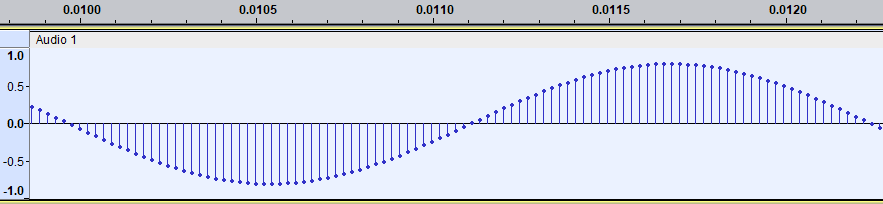
\includegraphics[width=0.5\textwidth]{../Images/sine_wave_representation_audacity.png}
    \caption{PCM representation of a sinusoidal signal}
    \label{fig:sine_wave_representation_audacity}
\end{figure}

Each vertical line represents a sample. The horizontal axis represents the time, and the vertical axis represents the amplitude. The sampling rate is usually 44100 Hz, 48000 Hz, or 96000 Hz.

\section{Sound Source Localization}

Sound Source Localization (SSL) is the process of determining the position of a sound source. It usually uses a microphone array that captures the sound signals from multiple directions. Various applications use SSL \cite{Grumiaux_2022}, such as speech recognition \cite{7952261}, source separation \cite{8903121}, human-robot interaction \cite{Li_2016} or room acoustic analysis \cite{amengual}. In this thesis, SSL is used to estimate the distance and direction of a sound source to detect excessively noisy vehicles.

\subsection{Spectrograms for sound visualization}
\label{subsec:spectrograms}

Spectrograms are a visual representation of the frequency content of a sound signal. They are often used in sound source localization to identify the direction of a sound source. The spectrogram is a two-dimensional representation of the frequency content of a sound signal (figure \ref*{fig:spectrogram_example}).

\begin{figure}[H]
    \centering
    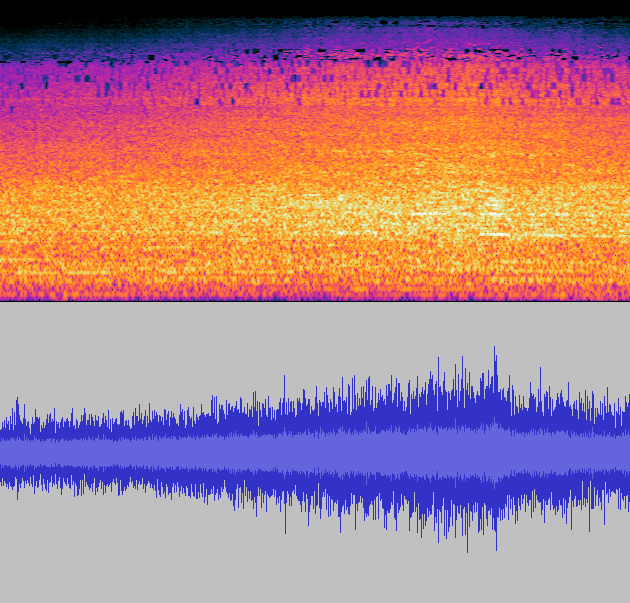
\includegraphics[width=0.5\textwidth]{../Images/spectrogram-example.png}
    \caption{Spectrogram of a sound signal}
    \label{fig:spectrogram_example}
\end{figure}

The x-axis represents time, and the y-axis represents frequency. The intensity of the color at each point in the spectrogram represents the amplitude of the frequency component. A matrix of spectrograms allows the representation of multiple channels, such as the ones recorded by a microphone array. On that matrix, each spectrogram represents the frequency content of a single channel (figure \ref*{fig:2_channel_spectrogram_example}).

\begin{figure}[H]
    \centering
    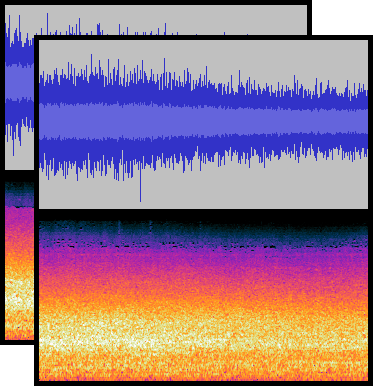
\includegraphics[width=0.4\textwidth]{../Images/2-channel-spectrogram-example.png}
    \caption{Dual channel spectrogram matrix of a sound signal}
    \label{fig:2_channel_spectrogram_example}
\end{figure}

Looking at the frequency content of the sound signal allows us to identify the time delta of a recorded sound by using a multi-channel spectrogram. The bright spot on the spectrogram will indicate a jump in the amplitude and determine the start time of the recording of a loud sound. By comparing this time with the other channel, we can find the direction of the sound source by comparing the sound signal's time delta with the other channels' time delta (figure \ref*{fig:spectrogram_offset}).

\begin{figure}[H]
    \centering
    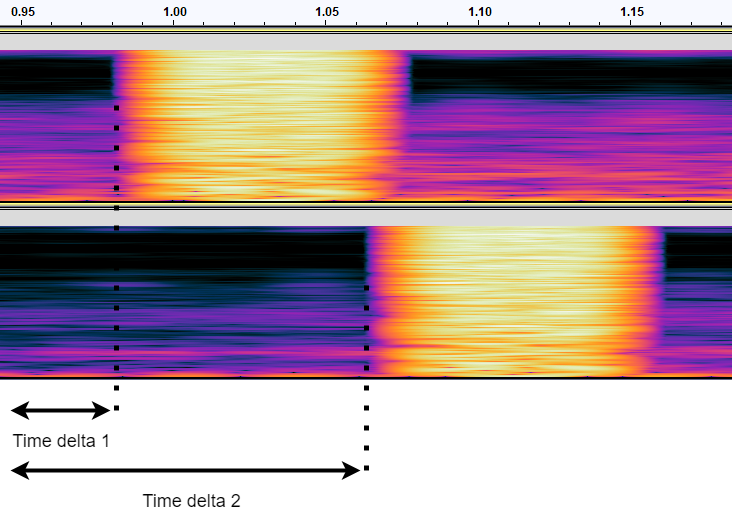
\includegraphics[width=0.5\textwidth]{../Images/time_delta.png}
    \caption{Spectrogram of two sound signals with time their delta}
    \label{fig:spectrogram_offset}
\end{figure}

Since we know the distance between the microphones, we can determine the direction of the sound.

\subsection{Origin of sound using two microphones}

Admitting the following setup (figure \ref*{fig:microphones_setup}), if the time delta 1 is greater than the time delta 2 of the other channels (setup 1), the sound source is closer to microphone 2. If the time delta 1 equals the time delta 2 (setup 3), the sound source is at the same distance to both microphones. If the time delta 2 is greater than the time delta 1 (setup 2), the sound source is closer to the microphone 1. 

\begin{figure}[H]
    \centering
    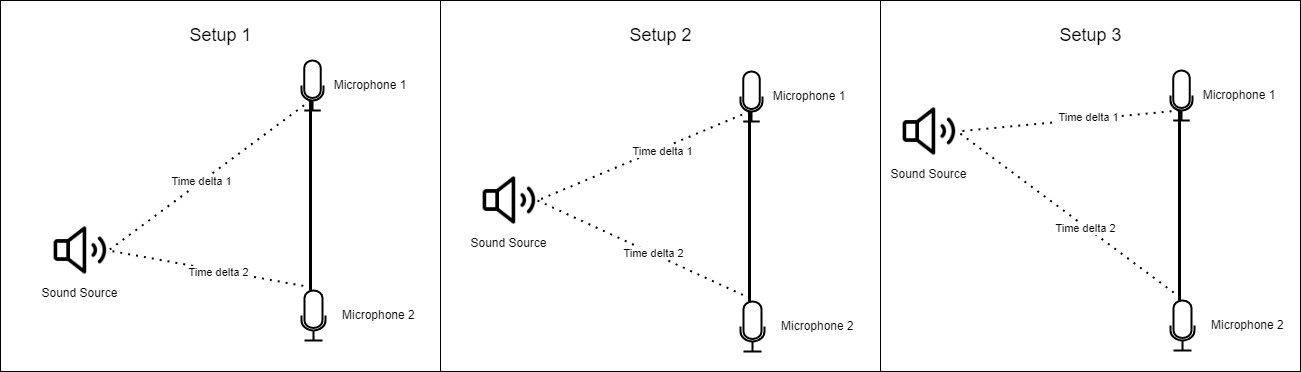
\includegraphics[width=1\textwidth]{../Images/microphones_setups.png}
    \caption{Sound source localization setup}
    \label{fig:microphones_setup}
\end{figure}

This concept can be formalized and is better explained in \cite{Scola2010DirectionOA}. Once the delay between the two microphones is known, the equation allows us to find the direction of the sound source by using trigonometric calculations. As in the figure \ref*{fig:sound-source-from-two-microphones}, considering point $M$ as the sound source and point $A$ and $B$ as microphones, the distance between the two microphones is $d$ and the time delta between the two microphones is $\Delta t$, the angle $\alpha$ can be calculated.

\begin{figure}[H]
    \centering
    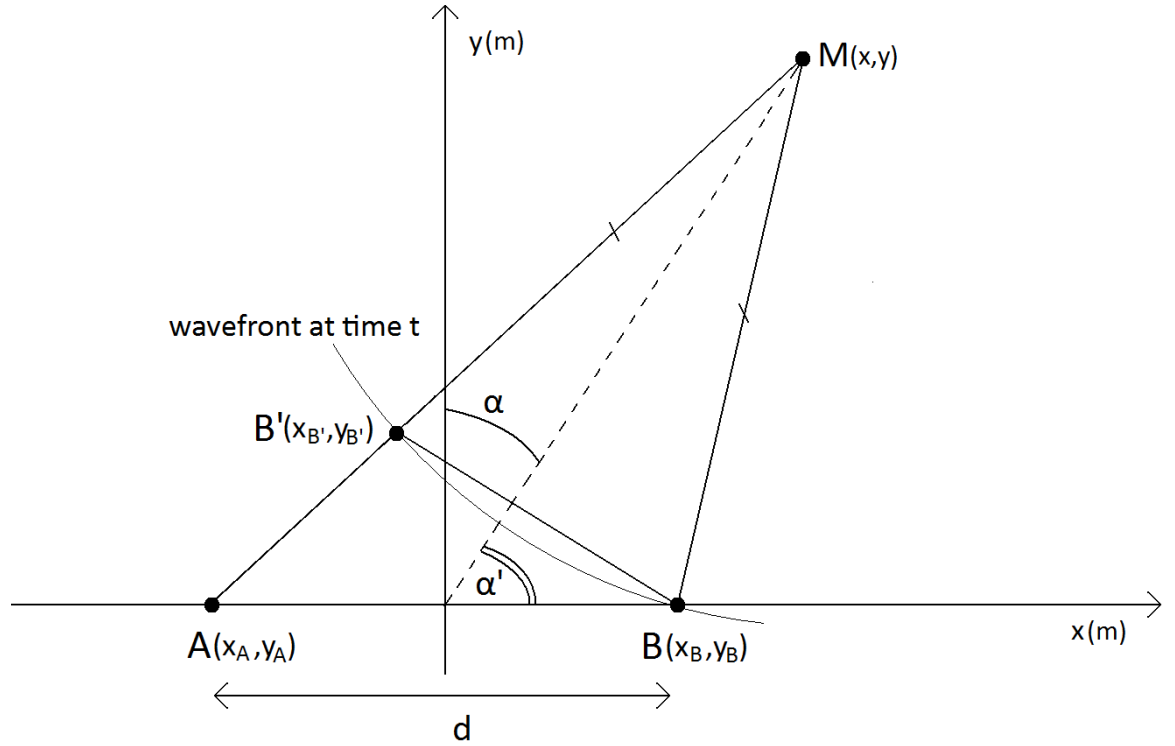
\includegraphics[width=0.7\textwidth]{../Images/sound-source-from-two-microphones.png}
    \caption{Equation formalization. Original image from \cite{Scola2010DirectionOA}}
    \label{fig:sound-source-from-two-microphones}
\end{figure}

Looking at the graphic allows us to find the following equation:

\begin{equation}
    AB' = AM-B'M
\end{equation}

With Pythagorean theorem: 

\begin{equation}
    AM = \sqrt{(X_{a}-X)^2 + (Y_{a}-Y)^2}
\end{equation}
\begin{equation}
    BM = \sqrt{(X_{b}-X)^2 + (Y_{b}-Y)^2}
\end{equation}

The two microphones have the same $Y$ coordinate, so $Y_{a} = Y_{b} = Y$ and $Y_{a}-Y_{b} = 0$ and $X_{a} = -X_{B}$ The equation becomes:

\begin{equation}
    y = \pm\sqrt{\frac{AB'^2}{4} - x^2_{B} + x^2(\frac{4\cdot x^2_{B}}{AB'^2} - 1)}
\end{equation}

This setup shows that two microphones are enough to determine the direction of a sound source.
%!!!!!!! TODO - compléter la formalisation

\section{Neural networks}

Neural networks are machine learning algorithms based on biological neurons used to solve various problems, including image recognition, speech recognition, and natural language processing. Neural networks learn from provided data to solve a problem without explicitly programming the solution. Many domains, like self-driving cars, facial recognition, and medical imaging, achieve state-of-the-art results using neural network models. 

A neural network needs to be trained to solve a problem. The training consists of providing the neural network with examples to recognize patterns in the data. Once we finish the training, the model can solve the problem.

A neural network (figure \ref*{fig:neural_network}) is composed of multiple neurons (the circles) that are organized in layers and connected to the neurons in the previous and next layers. 

\begin{figure}[H]
    \centering
    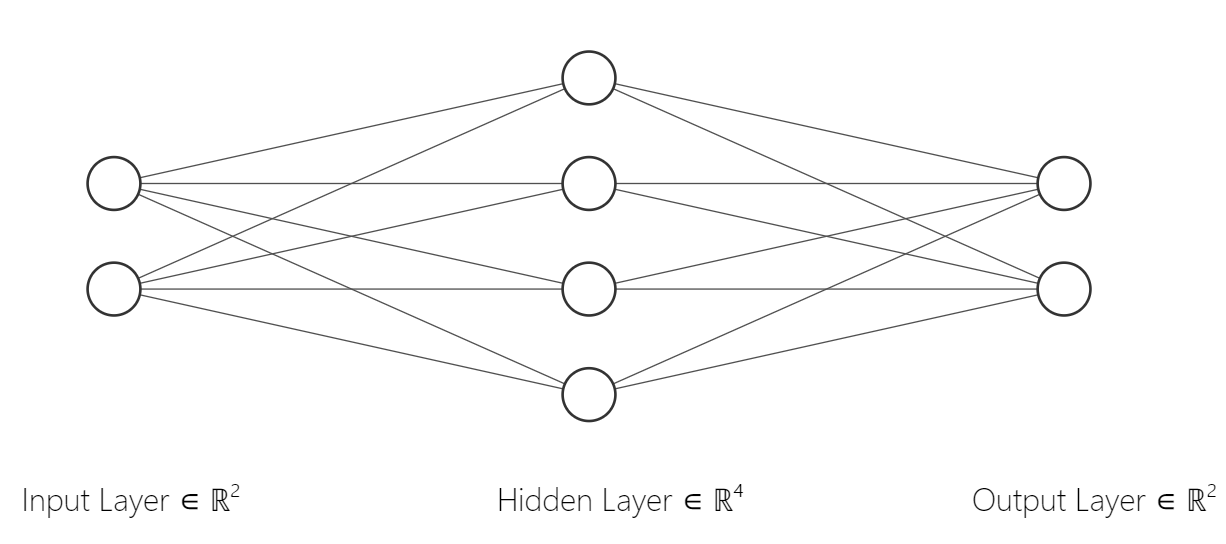
\includegraphics[width=0.7\textwidth]{../Images/neural_network_example.png}
    \caption{Neural network}
    \label{fig:neural_network}
\end{figure}

There are two main phases in the life of a neural network: training and inference. During the training phase, the neural network is trained on a large dataset of images. The neural network learns to recognize patterns in the images and classify them. During the inference phase, the neural network is used to classify new images.

Neural networks comprise multiple neurons. Neurons are mathematical functions with activation functions and weights. These determine how the neurons respond to inputs and connect to other neurons. Neural networks train themselves by adjusting the weights to minimize the error between the predicted and desired outputs. They use an optimization algorithm to adjust the neurons' weights \cite{sun2019optimization}. Multiple optimization algorithms exist, including gradient descent\cite{zhang2019gradient} and backpropagation\cite{Sekhar}. These algorithms minimize the error between the predicted and desired outputs.

%TODO - plagiat?
\subsection{Neuron}

A neuron is a mathematical function that takes multiple inputs and produces an output. The activation function and the weights of the neuron determine the output. The activation function determines how the neuron responds to inputs. The weights determine the importance of the inputs. The neuron's output is calculated by multiplying the inputs by their weights and applying the activation function to the result. The neuron sends its output to the next layer of neurons.

\paragraph{Activation function}

Multiple activation functions exist for neural networks. The most common activation functions are the linear function, the sigmoid function, the tanh function, and the ReLU function.

\begin{figure}[H]
    \centering
    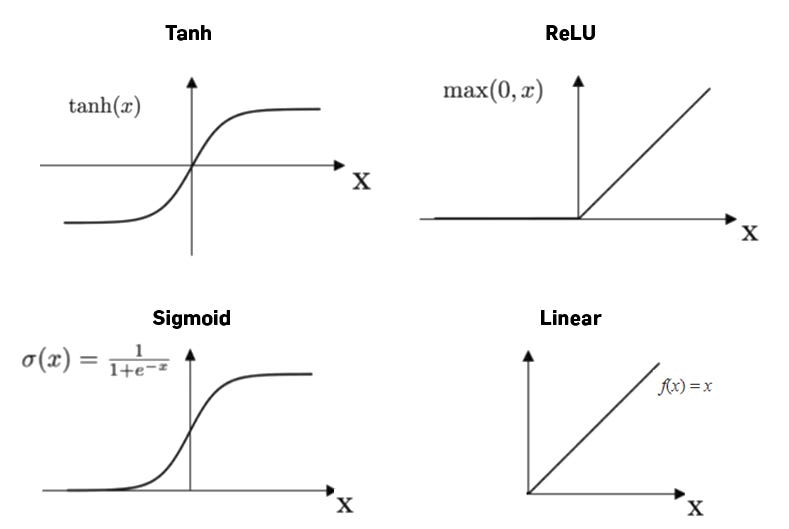
\includegraphics[width=0.7\textwidth]{../Images/activation_functions.png}
    \caption{Activation functions}
    \label{fig:activation_functions}
\end{figure}

These functions will determine how the neurons respond to inputs. These functions have been surveyed in [Activation Functions in Deep Learning: A Comprehensive Survey and Benchmark]\cite{dubey2022activation}. It shows that the ReLU function is the most used activation function in deep learning. The ReLU function is defined as:

\begin{equation}
    f(x) = max(0, x)
\end{equation}

The ReLU function is used in most neural networks because it is fast to compute and provides good results.

% TODO Vérifier les équations

\paragraph{Loss function}

Neural networks use a loss function to measure the error between the predicted and desired outputs. The loss function is a mathematical function that takes the predicted and desired outputs as inputs and outputs a value representing the error between the predicted and desired outputs. The optimization algorithms use the loss function to adjust the neurons' weights to minimize the error between the predicted and desired outputs. When the loss function's value is low, the neural network accurately predicts the desired outputs.


There is a wide variety of loss functions, including the mean squared error and the cross-entropy.

The mean squared error loss function is defined as follows:

\begin{equation}
    L(y, \hat{y}) = \frac{1}{n} \sum_{i=1}^{n} (y_{i} - \hat{y}_{i})^2
\end{equation}

Where $y$ is the desired output, $\hat{y}$ is the predicted output, and $n$ is the number of classes.

The cross-entropy loss function is defined as follows:

\begin{equation}
    L(y, \hat{y}) = - \sum_{i=1}^{n} y_{i} \cdot log(\hat{y}_{i})
\end{equation}

Where $y$ is the desired output, $\hat{y}$ is the predicted output, and $n$ is the number of classes.

We can add weights to the loss function to give more importance to some classes. It helps when a dataset is unbalanced by giving more importance to the underrepresented classes. The weighted cross-entropy loss function is defined as follows:

\begin{equation}
    L(y, \hat{y}) = - \sum_{i=1}^{n} w_{i} \cdot y_{i} \cdot log(\hat{y}_{i})
\end{equation}

Where $y$ is the desired output, $\hat{y}$ is the predicted output, $n$ is the number of classes, and $w$ is the weight of the class.

\paragraph{Gradient descent}

Gradient descent is an optimization algorithm that minimizes the error between the predicted and desired outputs. We use it to train neural networks. Gradient descent works by iteratively adjusting the neurons' weights to minimize the error between the predicted and desired outputs. It uses the gradient of the loss function to find the direction of the steepest descent. The weights are adjusted in the opposite direction of the gradient. The gradient descent algorithm is defined as follows:

\begin{equation}
    \theta_{n+1} = \theta_{n} - \alpha \cdot \nabla f(\theta_{n})
\end{equation}

Where $\theta_{n}$ is the current weight, $\alpha$ is the learning rate, and $\nabla f(\theta_{n})$ is the gradient of the loss function. This algorithm is repeated until the loss function's value is low enough. The gradient descent algorithm is slow because it uses the entire dataset to compute the gradient of the loss function.

\paragraph{Mini-batch gradient descent}

Mini-batch gradient descent is a variant of gradient descent. It uses a batch of samples to compute the gradient of the loss function. It is faster than full gradient descent because it uses a mini-batch of samples instead of the entire dataset. It is also more stable than gradient descent because it uses a mini-batch of samples instead of a single sample. The mini-batch gradient descent algorithm is defined as follows:

\paragraph{Backpropagation}

Backpropagation is another optimization algorithm used to train neural networks. Gradient descent forms the basis of the backpropagation algorithm. It uses the gradient of the loss function to find the direction of the steepest descent. The weights are adjusted in the opposite direction of the gradient. Backpropagation is an iterative algorithm that adjusts the neurons' weights to minimize the error between the predicted and desired outputs. The backpropagation algorithm is defined as follows:

\begin{equation}
    \theta_{n+1} = \theta_{n} - \alpha \cdot \nabla f(\theta_{n})
\end{equation}

Where $\theta_{n}$ is the current weight, $\alpha$ is the learning rate, and $\nabla f(\theta_{n})$ is the gradient of the loss function.

\subsection{Neural network hyperparameters}
Neural networks use different hyperparameters to control the training process. The most common hyperparameters are the activation function and the learning rate.


\paragraph{Learning rate}

To train efficiently a neural network, we use a learning rate. It determines a factor of how much the weights are adjusted during training. A high learning rate will adjust the weights by a large amount, hence training the neural network faster but less precisely. A low learning rate will adjust the weights by a small amount, hence training the neural network slower but more precisely. The learning rate is a hyperparameter that needs to be tuned to achieve the best results.

A solution to this problem is to use an adaptive learning rate. Adaptive learning rates are learning rates that change during training. They are used to train the neural network faster and more precisely. [Adaptive Learning Rate and Momentum for Training Deep Neural Networks]\cite{hao2021adaptive} shows us how it can train neural networks efficiently without losing precision. 

\subsection{Deep Neural Networks}

Deep neural networks are a type of neural network composed of multiple layers of neurons\cite{Schmidhuber_2015}. They are trained on a large dataset of images and then used to classify new images. There are countless architectures \cite{LIU201711} and implementations of neural networks, but they all share the same basic principles. The most known architectures of neural networks include CNNs\cite{oshea2015introduction}, transformers\cite{vaswani2017attention}, and many others.

\subsection{Convolutional Neural Networks for sound source localization}
\label{sec:cnn_for_ssl}

Convolutional Neural Networks (CNNs)\cite{oshea2015introduction} are deep neural networks specifically used for image recognition. They often comprise convolutional, subsampling, and fully connected layers (Figure \ref*{fig:cnn_example}).
\begin{itemize}
    \item{} Convolutional layers are used to extract features from images. These features are then fed into fully connected layers to perform classification. Each convolutional layer comprises multiple filters convolved with the input image to produce a feature map. The model trains the filters to extract specific features from the input image.
    \item{} Subsampling layers are used to reduce the size of the feature maps. The most common subsampling layer is the max-pooling layer, which takes the maximum value of a specific region of the feature map.
    \item{} Fully connected layers are trained to classify the features extracted by the convolutional layers. The output of the fully connected layers is a probability distribution over the possible classes. 
\end{itemize}

\begin{figure}[H]
    \centering
    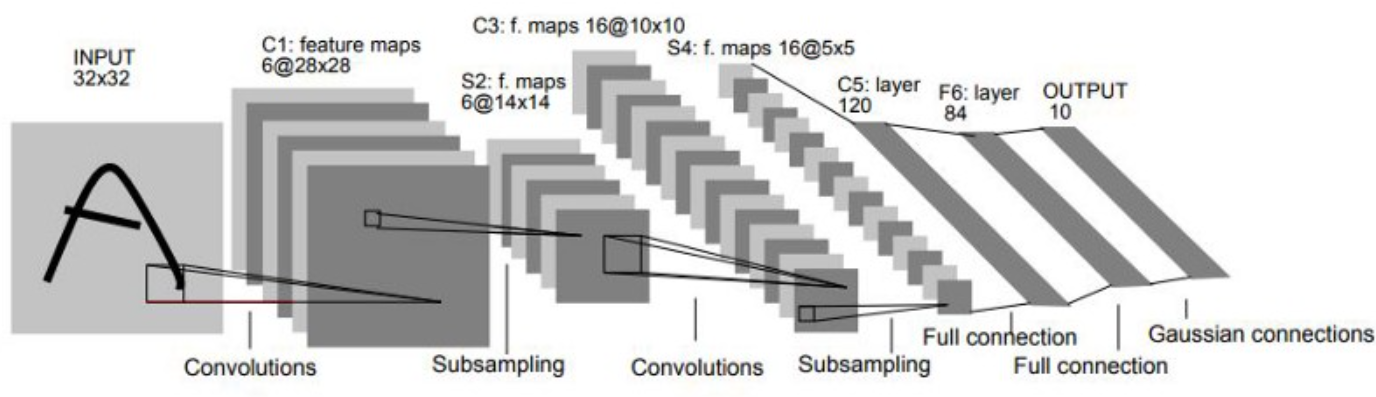
\includegraphics[width=0.7\textwidth]{../Images/cnn_example.png}
    \caption{CNN architecture example with LeNet-5 \protect\cite{726791} composed of two convolutional layers, two subsampling layers, and finishing with two fully connected layers.}
    \label{fig:cnn_example}
\end{figure}

Even if CNNs are mainly used to classify real-life photography, they can classify any image, including sounds. The report [A survey of sound source localization with deep learning methods]\cite{Grumiaux_2022} shows that deep neural networks achieve good scores in sound source localization. CNNs can use any image as input. Based on section \ref*{subsec:spectrograms}, we can use the spectrograms as input in the network since we convert the sound into images during the spectrogram process. An approach for sound source localization is to use zones from which the sound can come as classes. The CNN will output a probability distribution over the possible classes. The class with the highest probability is the predicted class. The predicted class can then refer to a zone. The CNN then outputs a probability distribution over the possible classes. The possible classes need to be defined before training the CNN. In\cite{s20010172}, they approach the problem with 15 classes, using angles 0, 30, and 60 degrees and distances 1, 2, and 3 meters (Figure \ref*{fig:Yiwere_classes}).

\begin{figure}[H]
    \centering
    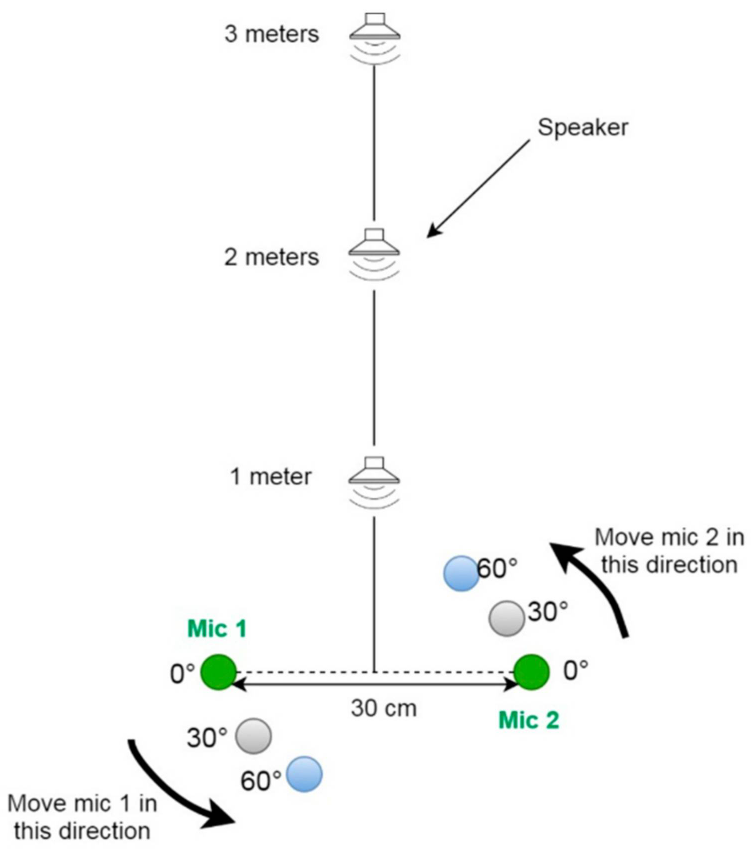
\includegraphics[width=0.5\textwidth]{../Images/Yiwere_classes.png}
    \caption{CNN for source localization}
    \label{fig:Yiwere_classes}
\end{figure}

This setup gives nine classes representing a different zone from where the sound can come from. The CNN will output a probability distribution over the nine classes, which allows determining the zone from where the sound comes from.

\subsection{Dropout layers}

Dropout layers are used to prevent overfitting in neural networks. 

\subsection{Transfer learning}

%!!!!!!! TODO - réécrire la partie sur le transfer learning
Transfer learning is a machine learning technique where a model trained on a specific task is reused as the starting point for a model on a different task. The model is trained on a large dataset and then used as a starting point for a model on a different dataset. The model is then trained on the new dataset, and the weights are adjusted to minimize the error between the predicted and desired outputs. Transfer learning is used to train models on smaller datasets and achieve better results than training the model from scratch.


\section{Datasets for machine learning}

Datasets are needed to train and test neural networks. They are composed of data and labels. The data is the neural network input, and the label is the expected output. Each entry in the dataset is composed of the data and the corresponding label. An entry in a dataset can also be called a sample. 

A balanced dataset contains nearly the same number of samples for each class. An unbalanced dataset contains a considerably different number of samples for each class.

\subsection{Datasets for sound source localization}
\label{sec:datasetsSSL}

In the case of sound source localization, the data is audio, and the labels are the zones of the sound source. 

Multiple datasets exist in sound source localization for neural networks. The most common are the DCASE 2019 task 3 dataset\cite{Adavanne2019_DCASE} and the DCASE 2020 task 3 dataset\cite{politis2020dataset}. These datasets are composed of audio files and the corresponding labels. The labels are the zones of the sound source. The audio files are recorded in a room with a microphone array and a sound source. The sound source is moved around the room, and the audio is recorded. The audio files are then annotated with the zones of the sound source. The annotations are done manually by listening to the audio files and annotating the zones. Multiple annotators then verify the annotations to ensure the quality of the annotations. 

Although these datasets are good baselines for sound source localization, they do not suit the needs of this project. The datasets are recorded in a closed environment and do not reflect the baseline defined in this project. Still, these datasets are good baselines for sound source localization and help to understand how to create a dataset.

\subsection{Dataset augmentation for audio classification}
% TODO add sources
Since recording many audio files is time-consuming and costly, and since the dataset needs to be large to train a neural network, we decided to use dataset augmentation techniques.

Dataset augmentation is a technique used to increase the size of a dataset. It is used to improve the performance of a neural network by training on more data, thus becoming better at generalizing. The most common techniques are flipping, rotating, and cropping images, but since the classification in this project is realized on audio, other techniques are needed to augment the dataset. 

Some techniques that work well on audio are adding noise, changing the pitch, or simulating new data. 

\section{Dataset generation using simulation}
\label{sec:dataset_generation_simulation}

Simulating a dataset is a technique used to create a dataset without recording data from real life. It helps to create a dataset with many samples. Since the goal is to generate sounds in an open environment, a 3D-capable engine is necessary. Game engines are increasingly popular for simulation tasks since they are optimized for real-time rendering and can simulate complex 3D scenes. The game engine must simulate sound propagation for a realistic audio simulation. 

TODO

% TODO





\subsection{Metrics review for neural networks}

\paragraph{Accuracy}
The most common metric for neural networks is the accuracy. The accuracy is the number of correct predictions divided by the total number of predictions. Accuracy is a good metric for classification problems since it tells us how the model performs. The accuracy is defined as follows:

\begin{equation}
    \text{Accuracy} = \frac{\text{Number of correct predictions}}{\text{Total number of predictions}}
\end{equation}

The accuracy is a useful metric for classification problems as it provides insight into how well the model performs. However, it may not be the best metric for unbalanced datasets. For instance, if a dataset contains 90\% of class A and 10\% of class B, a model that always predicts class A will have an accuracy of 90\%. Although this model has high accuracy, it is ineffective since it always predicts the same class.

\paragraph{Recall}
The recall is another metric that can be used. The recall is the number of true positives divided by the number of true positives and false negatives. The recall is defined as follows:

\begin{equation}
    \text{Recall} = \frac{\text{True positives}}{\text{True positives} + \text{False negatives}}
\end{equation}

The recall is a good metric for unbalanced datasets since it considers the number of false negatives.

\paragraph*{F1 score}
Another metric that can be used is the F1 score. The F1 score is the harmonic mean of the precision and recall. The F1 score is defined as follows:

\begin{equation}
    \text{F1 score} = 2 \times \frac{\text{Precision} \times \text{Recall}}{\text{Precision} + \text{Recall}}
\end{equation}

The F1 score is a good metric for unbalanced datasets since it considers precision and recall. 

\paragraph*{Confusion matrix}

To have a visual understanding of how a model performs, a confusion matrix can be used. A confusion matrix is a matrix that shows the number of correct and incorrect predictions for each class. The confusion matrix can be used with any number of classes and is a good way to visualize the performance of a model. The main aim of the visualization of a confusion matrix is to see which classes are misclassified and which classes are correctly classified. For example, in a binary classification problem, the confusion matrix is a 2x2 matrix. The confusion matrix is defined as follows:

\begin{equation}
    \begin{bmatrix}
        \text{True positive} & \text{False negative} \\
        \text{False positive} & \text{True negative}
    \end{bmatrix}
\end{equation}

And the matrix can be visualized as follows:

\begin{figure}[H]
    \centering
    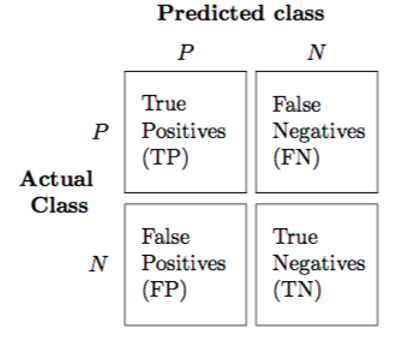
\includegraphics[width=0.5\textwidth]{images/confusion_matrix_example.png}
    \caption{Confusion matrix visualization}
    \label{fig:confusion_matrix}
\end{figure}

The confusion matrix allows us to understand which classes are misclassified and to better understand if there are difficulties for the model to predict certain classes.


\section{Sound propagation}
Sound propagation is the physical process by which sound waves propagate in a given environment. Multiple factors affect the propagation of sound waves, including reverberation, occlusion, doppler effect, and obstruction.


The strength of the sound wave depends on various factors, including the frequency, environment, and distance from the sound source. These factors make an accurate identification and localization of a sound source difficult; thus, we need a more accurate and robust sound source localization system.

\subsection{Microsoft Project Acoustics}

Microsoft Project Acoustics is a sound propagation engine that simulates the propagation of sound waves in a given environment. Various applications, including video games, virtual reality, and physics simulation, use this engine. It simulates wave effects like obstruction, reverberation, and occlusion in complex 3D scenes without requiring zone markup or raytracing. It works similarly to a raytracing engine but is precomputed and optimized for real-time performance. 

\subsubsection{Sound Propagation in game-engine}

\section{Adversarial Attacks}
\label{sec:adversarial_attacks}

Adversarial attacks are a manipulation technique that aims to fool a neural network by modifying the input data. The goal is to make the neural network misclassify. Adversarial attacks allow us to test the robustness of neural networks and understand how neural networks work and how we can improve them.

Adversarial attacks can be categorized into white-box attacks and black-box attacks. White-box attacks are attacks where the attacker has access to the neural network's parameters and architecture. Conversely, black-box attacks are attacks where the attacker cannot access the neural network's parameters and architecture.

One of the most common adversarial attacks is the Fast Gradient Sign Method (FGSM)\cite{goodfellow2015explaining}. It is a white-box attack that uses the gradient of the loss function to find the adversarial example. The adversarial example is calculated using the following equation:

\begin{equation}
    X_{adv} = X + \epsilon \cdot sign(\nabla_{X}J(\theta, X, y))
\end{equation}

$X$ is the input, $y$ is the target class, $\epsilon$ is the magnitude of the perturbation, and $J(\theta, X, y)$ is the loss function. The loss function is the function that the neural network normally tries to minimize, but here is used to maximize the loss. The gradient of the loss function is calculated for the input $X$. The sign of the gradient is then calculated and multiplied by the magnitude of the perturbation $\epsilon$. The result is added to the input to create the adversarial example $X_{adv}$. The adversarial example is then fed into the neural network, which outputs the adversarial class (Figure \ref*{fig:fgsm}).

\begin{figure}[H]
    \centering
    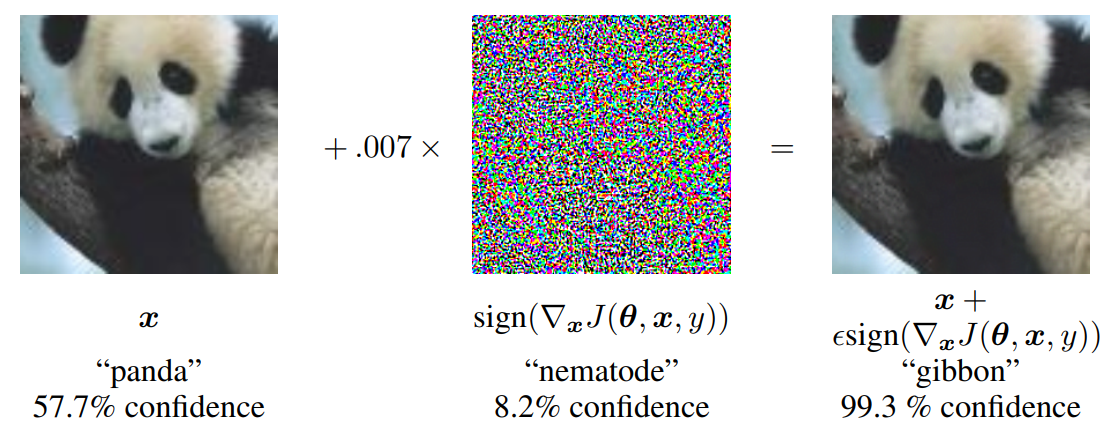
\includegraphics[width=0.7\textwidth]{../Images/fgsm.png}
    \caption{FGSM example in \cite{goodfellow2015explaining} with a neural network classifying a panda as a gibbon because of the attack.}
    \label{fig:fgsm}
\end{figure}

\subsection{Signal estimation from Short Time Fourier Transform}

The Griffin-Lim algorithm\cite{6701851} is an iterative algorithm that uses a spectrogram to estimate the phase of an audio signal. The algorithm starts with a random phase and iteratively updates the phase until the spectrogram converges to the original spectrogram. The algorithm is defined as follows:

% TODO ajouter l'algo